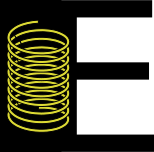
\includegraphics[height=1.25cm]{images/pictograms/elasticity}

\includegraphics[height=1.25cm]{images/pictograms/benchmark}

\includegraphics[height=1.25cm]{images/pictograms/FEM}

\includegraphics[height=1.25cm]{images/pictograms/3d}

%%%%%%%%%%%%%%%%%%%%%%%%%%%%%%%%%%%%%%%%%%%%%%%%%%%%%%%%%%%%%%%%%%%%%%%%%%%%%%%%%%%%%%%%%%%%%%%%%%%

\lstinputlisting[language=bash,basicstyle=\small]{python_codes/fieldstone_90/keywords.key}

\begin{center}
Code at \url{https://github.com/cedrict/fieldstone/tree/master/python_codes/fieldstone_90}
\end{center}

\par\noindent\rule{\textwidth}{0.4pt}

%%%%%%%%%%%%%%%%%%%%%%%%%%%%%%%%%%%%%%%%%%%%%%%%%%%%%%%%%%%%%%%%%%%%%%%%%%%%%%%%%%%%%%%%%%%%%%%%%

This axisymmetric elastic probem is common in the literature, see for 
instance Sadd \cite{sadd14}. A hollow thick-walled cylinder is placed under the
action of uniform internal and external pressure loadings, as shown here:

\begin{center}
\includegraphics[width=4cm]{python_codes/fieldstone_90/images/sadda}\\
{\captionfont Taken from Sadd \cite{sadd14}}
\end{center}


\section*{Analytical solution}

One can easily show that the stress components are such that
\begin{eqnarray}
\sigma_{rr} &=& \frac{A}{r^2} + B \\
\sigma_{\theta\theta} &=& -\frac{A}{r^2} + B
\end{eqnarray}
Applying the boundary conditions 
$\sigma_r(r_1)=-p_1$ and $\sigma_r=-p_2$ 
creates two equations
for the two unknown constants $A$ and $B$. 
Solving for these constants gives the result
\begin{eqnarray}
A &=& \frac{r_1^2r_2^2(p_2-p_1)}{r_2^2-r_1^2} \\
B &=& \frac{r_1^2p_1-r_2^2p_2 )}{r_2^2-r_1^2} 
\end{eqnarray}
Substituting these values back into relations above gives the final result for the stress field.

Taking $r_1=0.5$, $r_2=1$, $p_2=0$ and $p_1=p$, we can plot these:
\begin{center}
\includegraphics[width=6cm]{python_codes/fieldstone_90/images/saddb}\\
{\captionfont Taken from Sadd \cite{sadd14}}
\end{center}

Using the strain-displacement relations and Hooke's law, the radial
displacement is easily determined as
\[
u_r = \frac{1+\nu}{E}r \left[ (1-2\nu) B - \frac{A}{r^2}\right]
\]
Looking at the solution, we see that 
the stress field does not depend on the elastic constants, although the
resulting displacements do depend on both $E$ and $\nu$.
\begin{eqnarray}
\varepsilon_{rr} &=& \frac{\partial u_r}{\partial r} = 
\frac{1+\nu}{E} \left[ (1-2\nu) B + \frac{A}{r^2}\right]
\\
\varepsilon_{\theta\theta} &=& \frac1r \frac{\partial u_\theta}{\partial \theta} + \frac{u_r}{r} 
=\frac{u_r}{r}  
=\frac{1+\nu}{E} \left[ (1-2\nu) B - \frac{A}{r^2}\right] 
\\
\varepsilon_{zz} &=& \frac{\partial u_z}{\partial z} = 0 
\end{eqnarray}
It then follows that 
\[
\sigma_{zz} = \lambda div(\vec{u}) + 2 \mu \varepsilon_{zz} = 
\lambda (\varepsilon_{rr} + \varepsilon_{\theta\theta})
\qquad
\text{and}
\qquad
\sigma_{rz} = 2 \mu \varepsilon_{rz} 
\]

\section*{Implementation}

We approach this problem by assuming that the cylinder is infinite in the direction perpendicular 
to the page. We have an obvious axisymmetry: 

\begin{center}
\includegraphics[width=4cm]{python_codes/fieldstone_90/images/cyl}
\includegraphics[width=7cm]{python_codes/fieldstone_90/images/cyl2}\\
\end{center}

The setup is then as follows:

\begin{center}
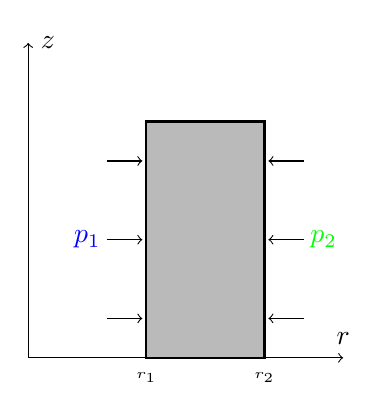
\begin{tikzpicture}
%\draw[fill=gray!23,gray!23](0,0) rectangle (6,5);
%\draw[step=0.5cm,gray,very thin] (0,0) grid (6,5); %background grid
\draw[thick,fill=gray!54] (2.5,.5)--(4,.5)--(4,3.5)--(2.5,3.5) -- cycle;

\draw[thin,->] (1,0.5) -- (5,0.5); %x
\draw[thin,->] (1,0.5) -- (1,4.5); %y
\node[] at (5,0.75) {$r$};
\node[] at (1.25,4.5) {$z$};

\node[] at (2.5,0.25) {\tiny $r_1$};
\node[] at (4,0.25) {\tiny $r_2$};

\draw[thin,->] (2,1) -- (2.45,1);
\draw[thin,->] (2,2) -- (2.45,2);
\draw[thin,->] (2,3) -- (2.45,3);

\draw[thin,->] (4.5,1) -- (4.05,1);
\draw[thin,->] (4.5,2) -- (4.05,2);
\draw[thin,->] (4.5,3) -- (4.05,3);

\node[] at (1.75,2) {\color{blue} $p_1$};
\node[] at (4.75,2) {\color{green} $p_2$};
\end{tikzpicture}
\end{center}

Because we have the analytical displacement field, we will be using it to 
impose Dirichlet boundary conditions on the sides, rather than pressure, and 
we will then recover strain and stress components.

Results for displacement, strain and stress as a function of $r$ are shown hereunder:
\begin{center}
\includegraphics[width=8cm]{python_codes/fieldstone_90/results/displacement.pdf}
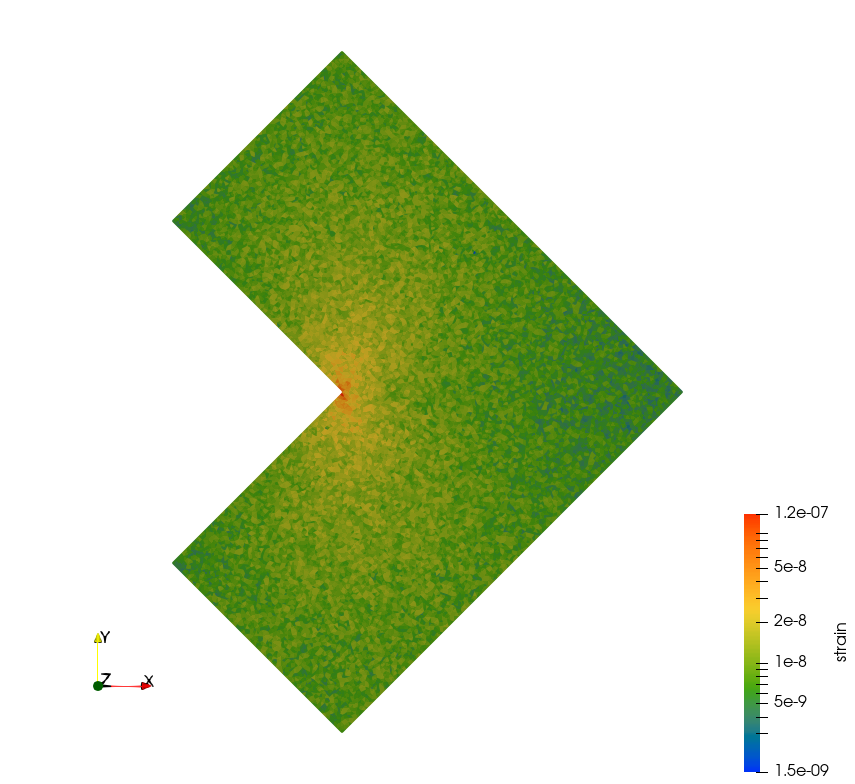
\includegraphics[width=8cm]{python_codes/fieldstone_90/results/strain.pdf}\\
\includegraphics[width=8cm]{python_codes/fieldstone_90/results/stress.pdf}
\end{center}
The match is perfect and shows that the axisymmetric formulation presented in 
Section~\ref{MMM-ss:fem_elast_axis} is correct.

ToDo: error calculations are not finished !

